%%%%%%%%%%%%%%%%%%%%%%%%%%%%%%%%%%%%%%%%% 
% Beamer Presentation
% LaTeX Template
% Version 1.0 (10/11/12)
% 
% This template has been downloaded from:
% http://www.LaTeXTemplates.com
% 
% License:
% CC BY-NC-SA 3.0 (http://creativecommons.org/licenses/by-nc-sa/3.0/)
% 
%%%%%%%%%%%%%%%%%%%%%%%%%%%%%%%%%%%%%%%%% 

% ----------------------------------------------------------------------------------------
%	PACKAGES AND THEMES
% ----------------------------------------------------------------------------------------

\newcommand{\norm}[1]{\left\lVert#1\right\rVert}
\newcommand{\abs}[1]{\left\lvert#1\right\rvert}

\documentclass{beamer}
\setbeamertemplate{caption}{\raggedright\insertcaption\par}

\mode<presentation> {

  \usetheme{Darmstadt}

  % \setbeamertemplate{footline} % To remove the footer line in all slides uncomment this line
  % \setbeamertemplate{footline}[page number] % To replace the footer line in all slides with a simple slide count uncomment this line

  \setbeamertemplate{navigation symbols}{} % To remove the navigation symbols from the bottom of all slides uncomment this line

  \addtobeamertemplate{navigation symbols}{}{%
    \usebeamerfont{footline}%
    \usebeamercolor[fg]{footline}%
    \hspace{1em}%
    \insertframenumber/\inserttotalframenumber
  }
}

\usepackage{graphicx} % Allows including images
\usepackage{booktabs} % Allows the use of \toprule, \midrule and \bottomrule in tables

% ----------------------------------------------------------------------------------------
%	TITLE PAGE
% ----------------------------------------------------------------------------------------

\title[Graph-Based Multimodal Data Processing]{Graph-Based Multimodal Data Processing} % The short title appears at the bottom of every slide, the full title is only on the title page

\author{Geoffrey Iyer} % Your name
\institute[UCLA] % Your institution as it will appear on the bottom of every slide, may be shorthand to save space
{
  University of California, Los Angeles \\ % Your institution for the title page
  GIPSA Lab, Universit\'{e} Grenoble Alpes \\
  \medskip
  \textit{gsiyer@math.ucla.edu} % Your email address
}
\date{November 14th, 2017} % Date, can be changed to a custom date

\begin{document}

\begin{frame}
  \titlepage % Print the title page as the first slide
\end{frame}

\begin{frame}
  \frametitle{Overview} % Table of contents slide, comment this block out to remove it
  \tableofcontents % Throughout your presentation, if you choose to use \section{} and \subsection{} commands, these will automatically be printed on this slide as an overview of your presentation
\end{frame}

% ----------------------------------------------------------------------------------------
% Notes to self: Idea for presentation.
% ----------------------------------------------------------------------------------------

% 1) Intro to multimodality
% 1a) Oh but it's hard to compare in general
% 2) Idea of distances and graphs
% 2a) graph laplacian
% 2b) ICIP paper
% 3) Graph matching

% ----------------------------------------------------------------------------------------
%	PRESENTATION SLIDES
% ----------------------------------------------------------------------------------------

% ------------------------------------------------
\section{Introduction \& Theory} % Sections can be created in order to organize your presentation into discrete blocks, all sections and subsections are automatically printed in the table of contents as an overview of the talk
% ------------------------------------------------

\subsection{Multimodality} % A subsection can be created just before a set of slides with a common theme to further break down your presentation into chunks

\begin{frame}
  \frametitle{Multimodal Datasets}
  With the increasing availability of data, many applications involve data drawn from more than one source (called \emph{modalities}).
  % 
  \begin{figure}
    \hfill
    \begin{minipage}[b]{0.38\linewidth}
      \centering
      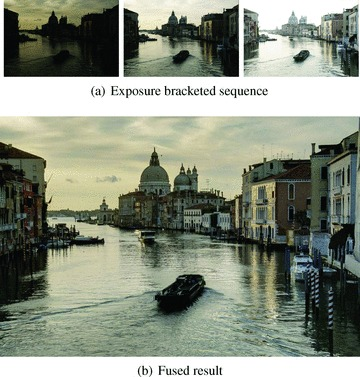
\includegraphics[width=\textwidth]{./Images/Exposure-Fusion.png}
      \caption{Exposure Fusion: \cite{Mertens2008}}
    \end{minipage}
    \hfill
    \begin{minipage}[b]{0.38\linewidth}
      \centering
      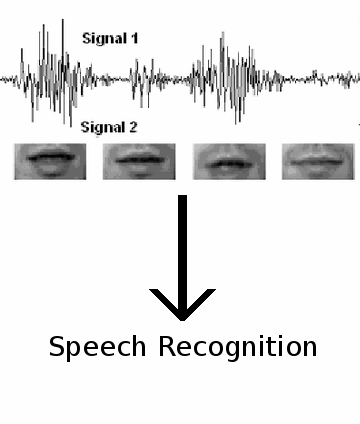
\includegraphics[width=\textwidth]{./Images/SpeechRecognitioncopy.png}
      \caption{Speech Recognition: \cite{Dactu2007}}
    \end{minipage}
    \hfill
  \end{figure}
\end{frame}
% ------------------------------------------------

\begin{frame}
  \frametitle{Example Multimodal Data}
  Remote sensing example: RGB + Elevation map.\\
  From 2015 IEEE Data Fusion Contest.\\
  \cite{DFC2015}\\
  \begin{figure}
    \hfill
    \begin{minipage}[b]{0.40\linewidth}
      \centering
      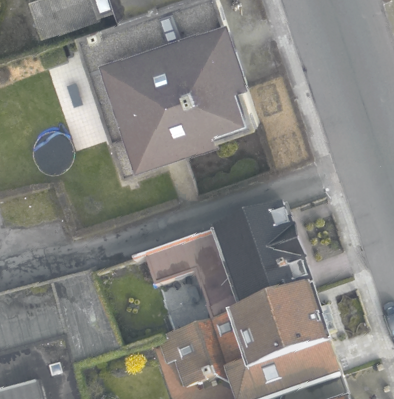
\includegraphics[width=\textwidth]{./Images/DFC2015/optical.png}
      \caption{RGB Data}
    \end{minipage}
    \hfill
    \begin{minipage}[b]{0.40\linewidth}
      \centering
      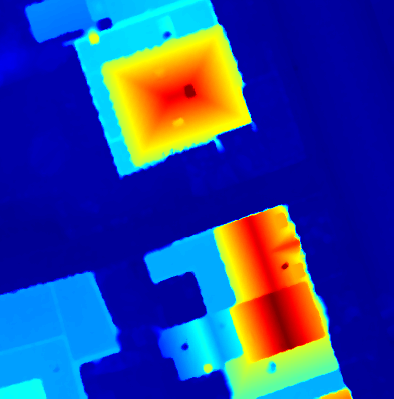
\includegraphics[width=\textwidth]{./Images/DFC2015/lidarColor.png}
      \caption{Lidar Data}
    \end{minipage}
    \hfill
  \end{figure}
\end{frame}
% ------------------------------------------------

\begin{frame}
  \frametitle{Challenges in Multimodality}
  Most multimodal methods are developed specifically for one problem, BUT: \\~\\
  %
  \cite{Lahat2015}: ``... a solution that is based on a sufficiently data-driven, model-free approach may turn out to be useful in very different domains.''\\~\\
  %
  Our approach: \\Represent data via a graph, compare graph representations.
\end{frame}

%-------------------------------------------------

%% More collecting of thoughts
% 1) Manifold laplacian is obviously important
% 1a) Fill in a few examples here!!
% 2) Graph laplacian approximates manifold laplacian
% 2a) I already have example with the disc. Maybe good enough?
% ?) Graph laplacian quadratic form gives graph function energy
%    I really need to explain this. What is function energy anyways?
%    Maybe think of it like the heat thingy. Dirichlet energy? No that's different.

\subsection{Graph Representation and Laplacian}
\begin{frame}
  \frametitle{Graph Representation: Background}
  For a dataset $X$ with $N$ elements \\~\\
  \hspace*{20pt} For each pair $x_i,x_j\in X$, define a \emph{weight} $w_{ij}\geq 0$ that\\  \hspace*{20pt} measures the similarity between the points. \\~\\
  \hspace*{20pt} $\implies$ represent data as $N \times N$ weight matrix $W$. \\~\\
  \hspace*{20pt} Common similarity measure from the literature: RBF kernel
  \[w_{ij} = \text{exp}\left(-\norm{x_i - x_j}^2 / \sigma \right).\]
  Get a representation of $X$ as a weighted graph $(V,E)$.
\end{frame}
  
%-------------------------------------------------

\begin{frame}
  \frametitle{Graph Laplacian}
  Perform analysis via the \emph{Graph Laplacian}\\ \cite{Chung1997}
  \[L = D - W.\]
  $D =$ diagonal degree matrix, $d_{ii} = \sum_{j=1}^N w_{ij}$.\\~\\
  View $L$ as an operator on the space of functions $f: V\to\mathbb{R}$.
  Related to the standard differential Laplacian $\Delta = \nabla^2$. \\~\\
%  \[Lf(v_i) = \sum_{j \neq i}w_{ij}\left(f(v_i) - f(v_j)\right).\]
  A manifold $\mathcal{M}$ can be discretized and represented by a graph. \\~\\
  Under mild assumptions and some renormalization, \\
  $L$ converges to $\Delta$ as mesh size $\to 0$.
\end{frame}

%-------------------------------------------------

\begin{frame}
  \frametitle{Graph Laplacian vs Differential Laplacian}
  Ex: A 1-D line graph. $L$ is related to the discrete Laplacian.
  \begin{figure}
    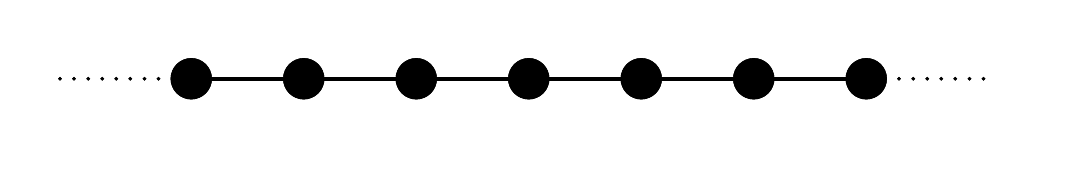
\includegraphics[width=\textwidth]{./Images/1dLaplacian/Graph.png}
  \end{figure}
  \vspace*{-5mm}
  \[L = \begin{bmatrix}
      \ddots & \vdots & \vdots & \vdots & \vdots\\
      \cdots &  2 & -1 &  0 &  0 & \cdots \\
      \cdots & -1 &  2 & -1 &  0 & \cdots \\
      \cdots &  0 & -1 &  2 & -1 & \cdots \\ 
      \cdots &  0 &  0 & -1 &  2 & \cdots \\ 
      &  \vdots & \vdots & \vdots & \vdots & \ddots \\
    \end{bmatrix}\]
  1-D discrete Laplacian with stepsize $h$:
  \[\Delta f(x) \approx \frac{-f(x-h) + 2\cdot f(x) - f(x+h)}{h^2}.\]
\end{frame}

%-------------------------------------------------
\begin{frame}
  \frametitle{Laplacian Eigenfunctions and Fourier Modes}
  Eigenfunctions of differential Laplacian give modes of vibration.\\
  Corresponding eigenvalues describe the energy of the state.\\~\\
  Ex: On the interval $[0,1]$, eigenfunctions are solutions to
  \[\Delta f = \frac{d^2f}{dx^2} = - \lambda f.\]
  \hspace*{20pt} These are exactly the normal Fourier modes
  \[\left\{\sin(k\pi x), \cos(\ell \pi x)\, :\, k \geq 1, \ell \geq 0\right\}.\]
  Eigenvectors of Graph Laplacian give a discrete version.\\
  Allow us to study symmetries and structure of the graph.
\end{frame}

%-------------------------------------------------

\begin{frame}
  \frametitle{Laplacian Eigenfunctions and Fourier Modes}
  Example: A disc in $\mathbb{R}^2$, and a graph representation.
  \setlength{\abovecaptionskip}{0pt plus 0pt minus 2pt} % Chosen fairly arbitrarily
  \setlength{\belowcaptionskip}{0pt plus 0pt minus 2pt} % Chosen fairly arbitrarily
  \begin{figure}
    \begin{minipage}[b]{0.18\linewidth}
      \centering
      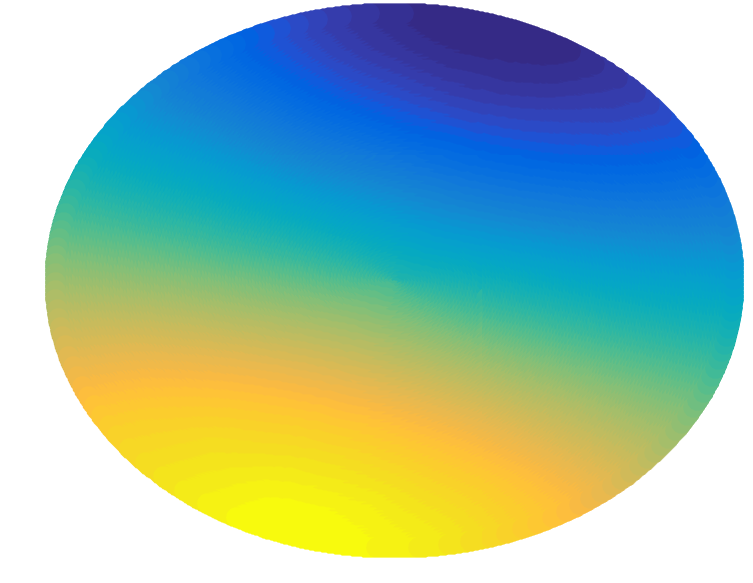
\includegraphics[width=\textwidth]{./Images/DiscExample/ManifoldLaplacian/evec02.png}
      \caption{\tiny $v_2$}
    \end{minipage}
    \hfill
    \begin{minipage}[b]{0.18\linewidth}
      \centering
      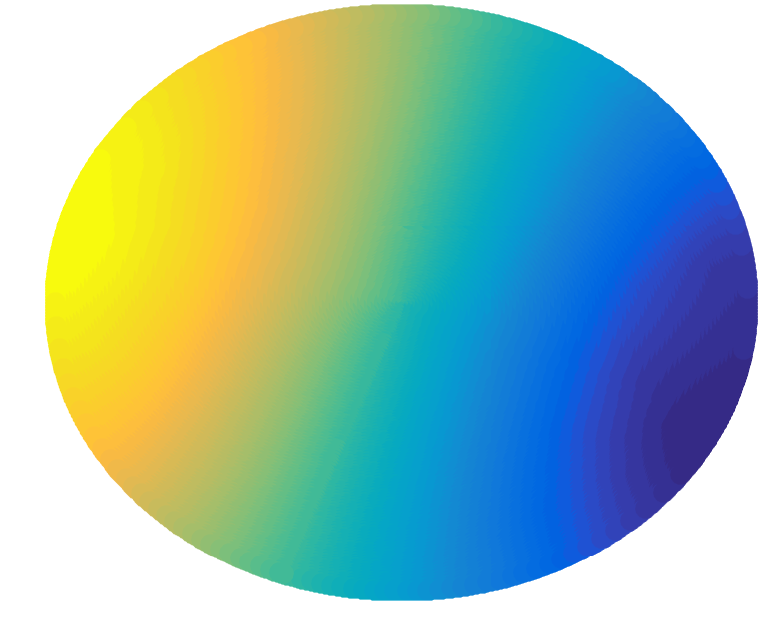
\includegraphics[width=\textwidth]{./Images/DiscExample/ManifoldLaplacian/evec03.png}
      \caption{\tiny $v_3$}
    \end{minipage}
    \hfill
    \begin{minipage}[b]{0.18\linewidth}
      \centering
      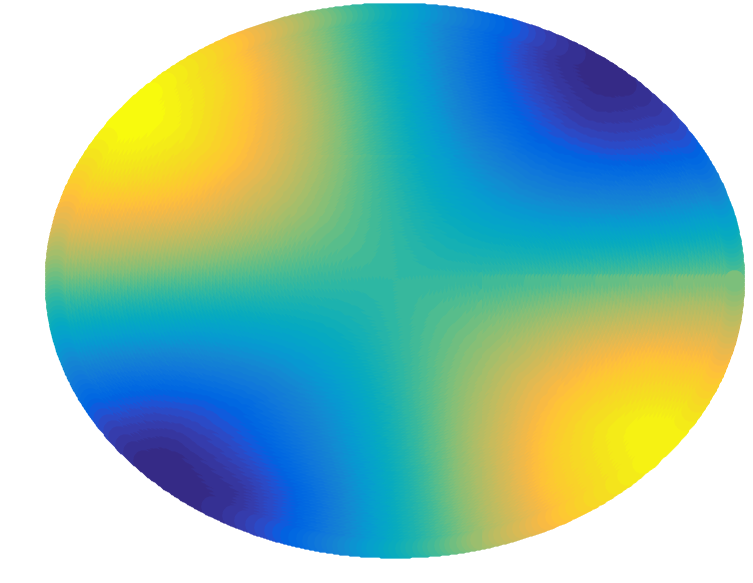
\includegraphics[width=\textwidth]{./Images/DiscExample/ManifoldLaplacian/evec04.png}
      \caption{\tiny $v_4$}
    \end{minipage}
    \hfill
    \begin{minipage}[b]{0.18\linewidth}
      \centering
      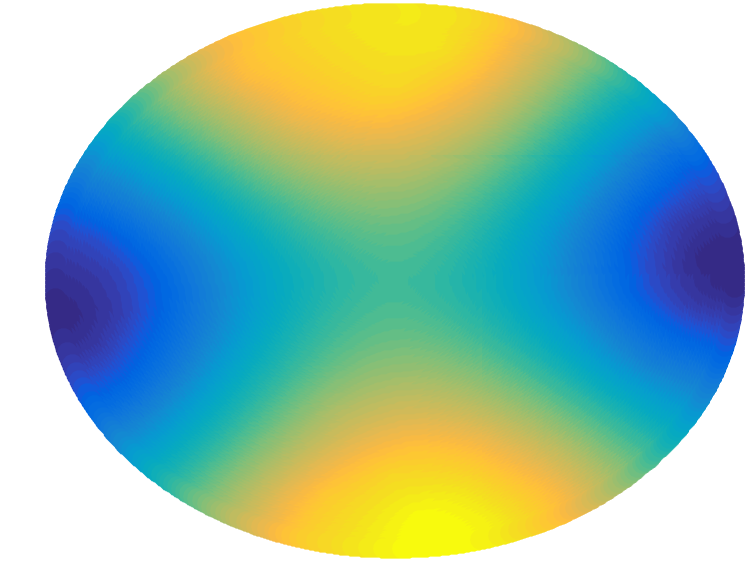
\includegraphics[width=\textwidth]{./Images/DiscExample/ManifoldLaplacian/evec05.png}
      \caption{\tiny $v_5$}
    \end{minipage}
    \hfill
    \begin{minipage}[b]{0.18\linewidth}
      \centering
      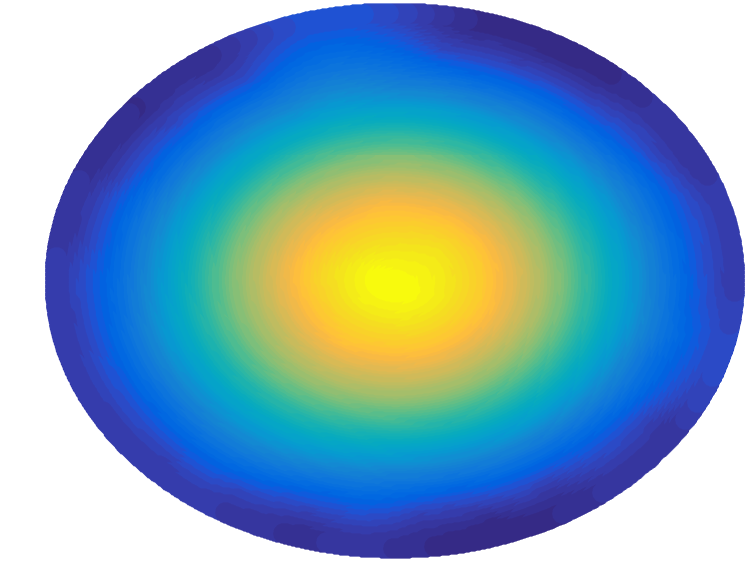
\includegraphics[width=\textwidth]{./Images/DiscExample/ManifoldLaplacian/evec06.png}
      \caption{\tiny $v_6$}
    \end{minipage}
    \caption{Differential Laplacian Eigenfunctions}
  \end{figure}
  \vspace*{-5mm}
  \begin{figure}
    \hfill
    \begin{minipage}[b]{0.18\linewidth}
      \centering
      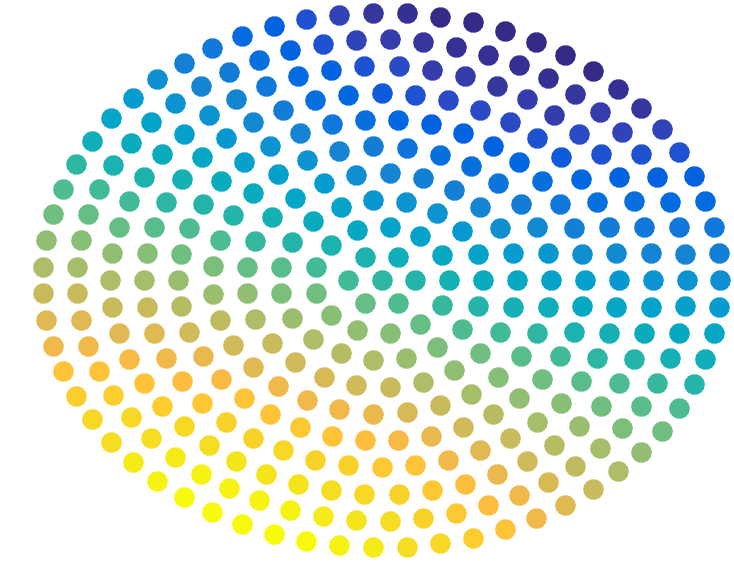
\includegraphics[width=\textwidth]{./Images/DiscExample/GraphLaplacian/evec02.png}
      \caption{\tiny $v_2$}
    \end{minipage}
    \hfill
        \begin{minipage}[b]{0.18\linewidth}
      \centering
      
\includegraphics[width=\textwidth]{./Images/DiscExample/GraphLaplacian/evec03.png}
      \caption{\tiny $v_3$}
    \end{minipage}
    \begin{minipage}[b]{0.18\linewidth}
      \centering
      
\includegraphics[width=\textwidth]{./Images/DiscExample/GraphLaplacian/evec04.png}
      \caption{\tiny $v_4$}
    \end{minipage}
    \hfill
    \begin{minipage}[b]{0.18\linewidth}
      \centering
      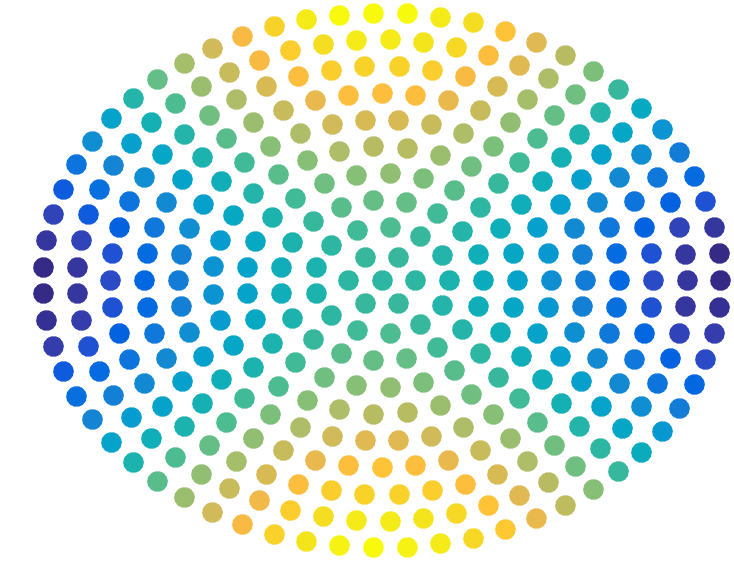
\includegraphics[width=\textwidth]{./Images/DiscExample/GraphLaplacian/evec05.png}
      \caption{\tiny $v_5$}
    \end{minipage}
    \hfill
    \begin{minipage}[b]{0.18\linewidth}
      \centering
      
\includegraphics[width=\textwidth]{./Images/DiscExample/GraphLaplacian/evec06.png}
      \caption{\tiny $v_6$}
    \end{minipage}
    \caption{Graph Laplacian Eigenvectors}
  \end{figure}
\end{frame}

%-------------------------------------------------

\begin{frame}
  \frametitle{Laplacian Eigenvectors and Fourier Modes}
  \begin{figure}
    \centering
    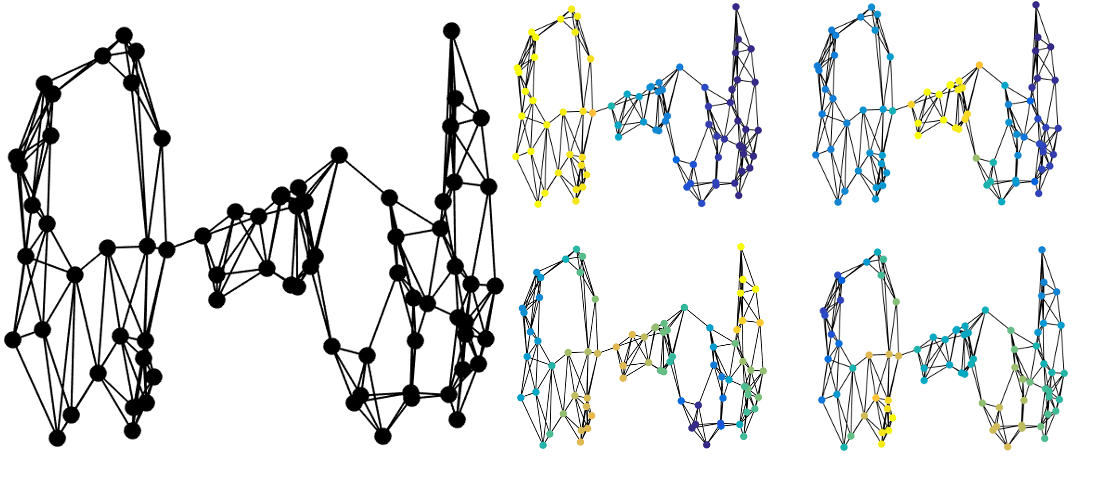
\includegraphics[width=\textwidth]{./Images/SyntheticGraph/combinedPic.png}
    \caption{Synthetic Graph and Example Eigenvectors}
  \end{figure}
\end{frame}

% ------------------------------------------------
\subsection{Laplacian Eigenvectors and Segmentation}
\begin{frame}
  \frametitle{Graph Min-Cut Problem}
  Graph Laplacian can also be understood via graph-cuts.\\
  Partition $V$ into $k$ sets $A_1,\ldots,A_k$ minimizing graph-cut energy.
  \[\text{Cut}(A_1,\ldots,A_k) = \frac{1}{2}\sum_{j=1}^kW(A_j,A_j^c).\]
  \[W(A,B) = \sum_{i \in A, j \in B} w_{ij}.\]
  \begin{figure}
    \centering
    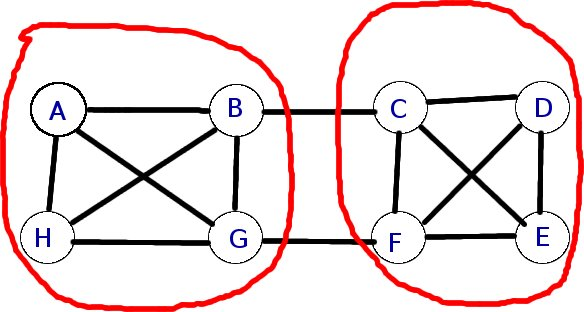
\includegraphics[width=0.6\textwidth]{./Images/graphMinCut.jpg}
  \end{figure}
\end{frame}

% ------------------------------------------------
\begin{frame}
  \frametitle{Graph Laplacian and Min-Cut}
  Notation: $u = \abs{V}\times k$ indicator matrix for $A_1,\ldots,A_k$.
  \[u_{ij} = \begin{cases} 1 &\text{if node $i$ is in set $A_j$} \\
      0 & \text{else}.
    \end{cases}\]
  Then \[Cut(A_1,\ldots,A_k) = \text{Tr}\left(u^TLu\right).\] \\
  So we rephrase our min-cut problem as:
  \[\text{argmin}_{u\text{ an indicator matrix}}\text{Tr}\left(u^TLu\right).\]
\end{frame}
% ------------------------------------------------

\begin{frame}
  \frametitle{Laplacian Eigenvectors and Min-Cut}
  Exact min-cut solution is computationally infeasible.\\~\\
  One popular relaxation: find
  \[\text{argmin}_{u^Tu = I}\text{Tr}\left(u^TLu\right).\]
  Solution: columns of $u$ are eigenvectors of $L$\\
  \hspace*{20pt}corresponding to smallest eigenvalues.\\~\\
  Heuristic \cite{vonLuxburg07}:
  \begin{align*}
    \text{eigenvectors of }L &\iff \text{ features extracted from data}
  \end{align*}

\end{frame}

% -------------------------------------------------
\begin{frame}
  \frametitle{Laplacian Eigenvectors and Min-Cut}
  Can use eigenvectors for a variety of applications. \\~\\
  %
  Ex: $K$-means on eigenvectors $\to$ segmentation:\\
  (called Spectral Clustering \cite{vonLuxburg07})
  %
  \begin{figure}
    \centering
    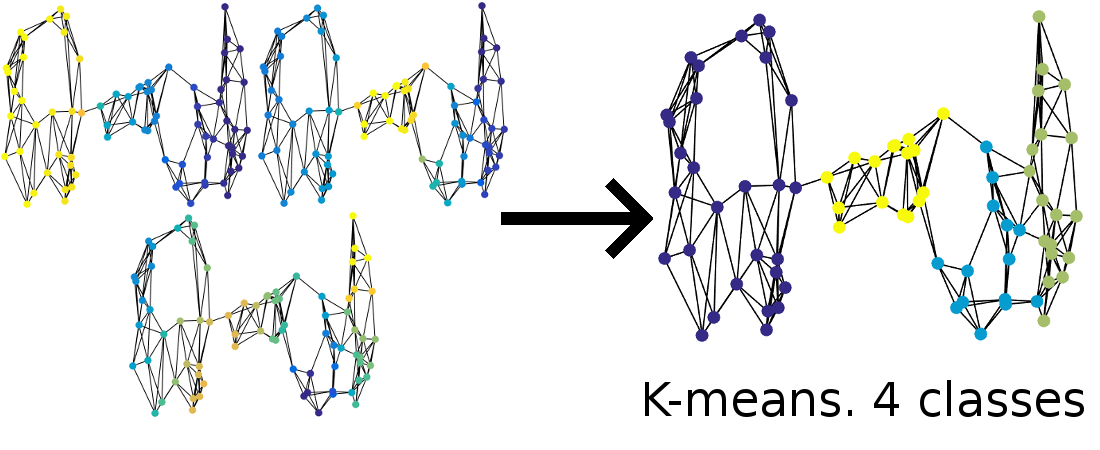
\includegraphics[width=\textwidth]{./Images/SyntheticGraph/combinedClassification.png}
  \end{figure}
\end{frame}

% -------------------------------------------------

\section{Multimodal Segmentation}
\subsection{Problem Setup}
\begin{frame}
  \frametitle{Problem Setup}
  Perform segmentation on \emph{coregistered}, multimodal datasets.\\ \cite{Iyer2017}
  \begin{figure}
    \hfill
    \begin{minipage}[b]{0.40\linewidth}
      \centering
      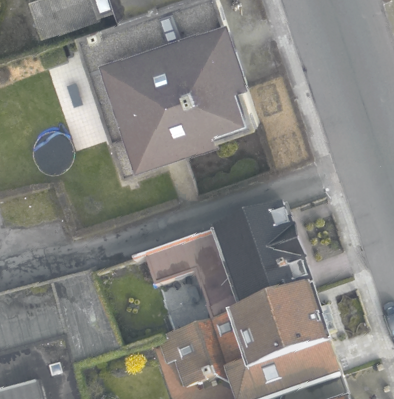
\includegraphics[width=\textwidth]{./Images/DFC2015/optical.png}
      \caption{RGB Data}
    \end{minipage}
    \hfill
    \begin{minipage}[b]{0.40\linewidth}
      \centering
      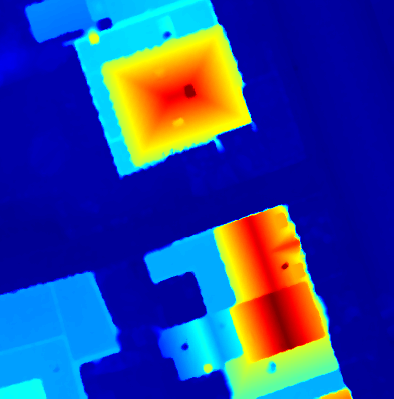
\includegraphics[width=\textwidth]{./Images/DFC2015/lidarColor.png}
      \caption{Lidar Data}
    \end{minipage}
    \caption{Example Multimodal Data}
  \end{figure}
\end{frame}

% ------------------------------------------------

\begin{frame}
  \frametitle{Problem Setup}
  From each modality, have a data set $X^k$. $N = \abs{X^1} = \cdots = \abs{X^k}$.\\~\\
  %
  From co-registration assumption: \\
  $i$-th point in $X^{k_1}$ corresponds to $i$-th point in $X^{k_2}$. \\~\\
  %
  $x_i^k = $ element $i$ from $X^k$.\\~\\
  For each modality $X^k$, calculate the distance matrix $E^k$ via
  \[E^k_{ij} = \norm{x^k_i - x^k_j}.\]
  %
  $\norm{\cdot}$ chosen based on the details of the modality.\\
  (often $\norm{\cdot}$ is the $L^2$-norm) \\~\\
  %
\end{frame}

% ------------------------------------------------

\begin{frame}
  \frametitle{Multimodal Weight Matrix}
  Scale each matrix by standard deviation (nondimensionalization)
  \[\bar{E}^k = \frac{E^k}{\text{std}\left(E^k\right)}.\]
  Define \[w_{ij} = \text{exp}\left(-\max\left(\bar{E}^1_{ij},\ldots,\bar{E}^k_{ij}\right)/\sigma\right).\]
  Using this weight matrix and Graph Laplacian theory, \\
  perform \emph{Spectral Clustering} and \emph{Semisupervised Graph MBO}\\
  \cite{Merkurjev13} to segment our datasets.\\~\\
\end{frame}

% ------------------------------------------------

\subsection{Synthetic Example}
\begin{frame}
  \frametitle{Synthetic Example: Data}
  \textbf{Why use max?}\\~\\
  Ground truth = 3 point clouds in $\mathbb{R}^3$ (100 points per cloud).\\
  Modality 1 = projection onto $xy$-plane.\\
  Modality 2 = projection onto $xz$-plane.\\
  Co-registration assumption: index is input to algorithm.
  \begin{figure}[ht]
    \begin{minipage}[b]{0.30\linewidth}
      \centering
      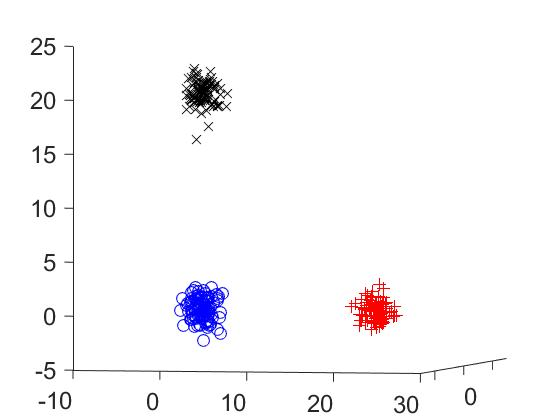
\includegraphics[width=\textwidth]{./Images/Synthetic/groundTruth.jpg}
      \caption{Underlying Data}
    \end{minipage}
    \begin{minipage}[b]{0.30\linewidth}
      \centering
      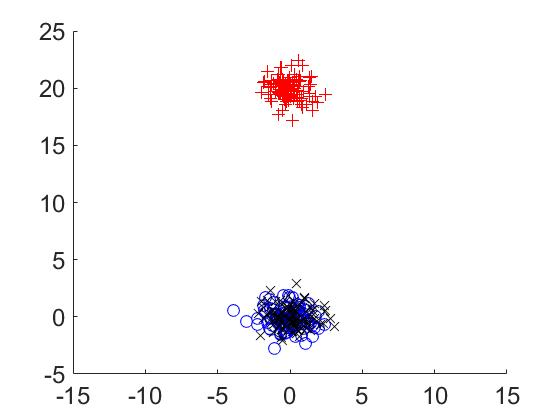
\includegraphics[width=\textwidth]{./Images/Synthetic/set1.jpg}
      \caption{Modality 1}
    \end{minipage}
    \begin{minipage}[b]{0.30\linewidth}
      \centering
      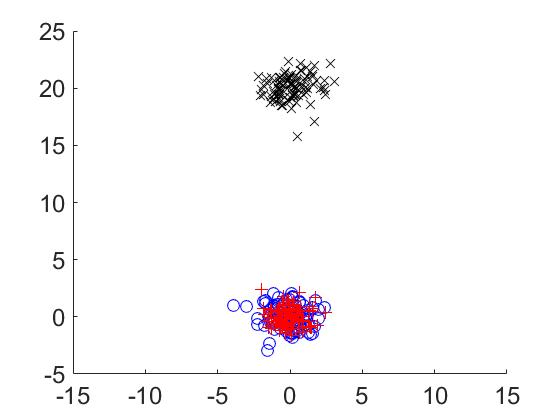
\includegraphics[width=\textwidth]{./Images/Synthetic/set2.jpg}
      \caption{Modality 2}
    \end{minipage}
    \label{fig:SynthData}
  \end{figure}
\end{frame}

% ------------------------------------------------

\begin{frame}
  \frametitle{Synthetic Example: Result of CCA}
  Result of CCA algorithm from \cite{Yeh2014}:\\~\\
  Both modalities are mapped to a common \emph{latent space}.\\
  (classification can then be done in this space.)
  \begin{figure}[ht]
    \begin{minipage}[b]{0.32\linewidth}
      \centering
      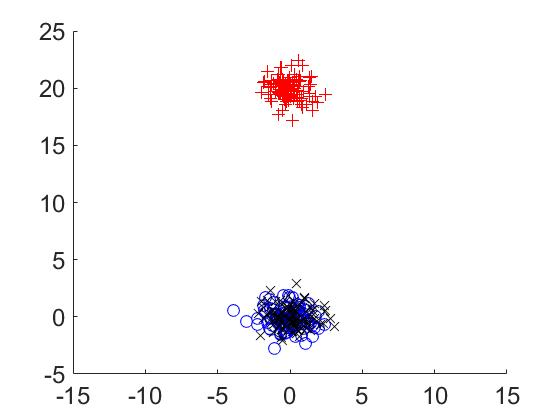
\includegraphics[width=\textwidth]{./Images/Synthetic/set1.jpg}
      \caption{Modality 1}
    \end{minipage}
    \begin{minipage}[b]{0.32\linewidth}
      \centering
      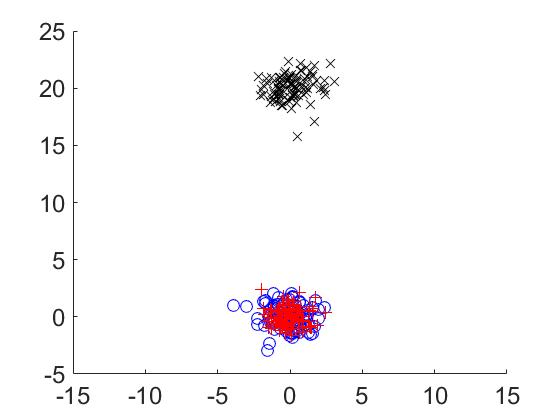
\includegraphics[width=\textwidth]{./Images/Synthetic/set2.jpg}
      \caption{Modality 2}
    \end{minipage}
    \begin{minipage}[b]{0.32\linewidth}
      \centering
      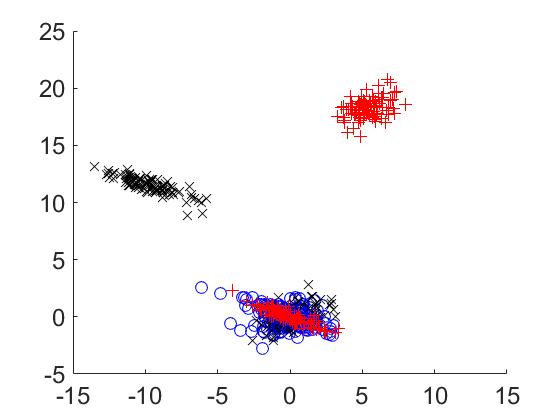
\includegraphics[width=\textwidth]{./Images/Synthetic/clustersLatent.jpg}
      \caption{Image in latent space}
    \end{minipage}
    \label{fig:SynthData}
  \end{figure}
\end{frame}

% ------------------------------------------------

\begin{frame}
  \frametitle{Synthetic Example: Result of Our Method}
  Result of our method:\\
  First 2 Laplacian Eigenvectors, plotted in $\mathbb{R}^2$.
  \begin{figure}
    \centering
    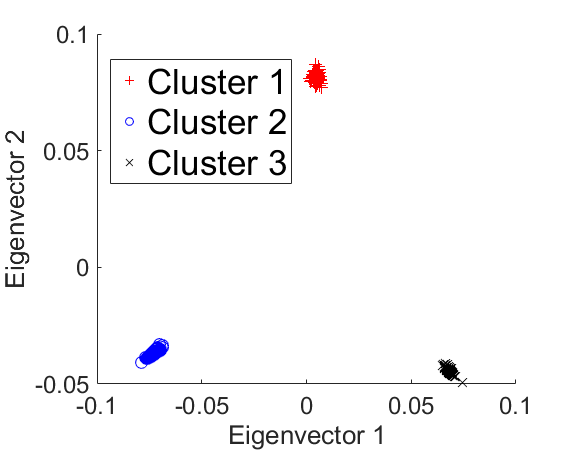
\includegraphics[width=0.5\linewidth]{./Images/Synthetic/clustersGraph.png}
    \caption{2 eigenvectors of graph Laplacian}
  \end{figure}
\end{frame}

% ------------------------------------------------

\subsection{Nystr\"{o}m Extension}
\begin{frame}
  \frametitle{Nystr\"{o}m Extension}
  As $\abs{X}$ becomes large, computing the $\abs{X}\times \abs{X}$ weight matrix $W$ becomes prohibitive. \\~\\
  Instead choose $A \subseteq X$ \emph{landmark nodes} with $\abs{A}\ll\abs{X}$. Up to permutation, we have
  \[  W = \begin{pmatrix} W_{A,A} & W_{A,A^c} \\ W_{A^c,A} & W_{A^c,A^c}
    \end{pmatrix}.\]
  \cite{Fowlkes04}: \\
  Approximate graph Laplacian eigenvectors using only $W_{A,A},W_{A^c,A}$.
  \[  W \approx \begin{pmatrix} W_{A,A} \\ W_{A^c,A} \end{pmatrix}
    W_{AA}^{-1} \begin{pmatrix} W_{A,A} & W_{A,A^c}\end{pmatrix}.\]
  Compute and store matrices of size at most $\abs{X}\times\abs{A}$.
\end{frame}

% ------------------------------------------------
\subsection{Results}
\begin{frame}
  \frametitle{DFC2015 Data}
  Our algorithm applied to DFC 2015\\ \cite{DFC2015}.
  \begin{figure}[ht]
    \begin{minipage}[b]{0.45\linewidth}
      \centering
      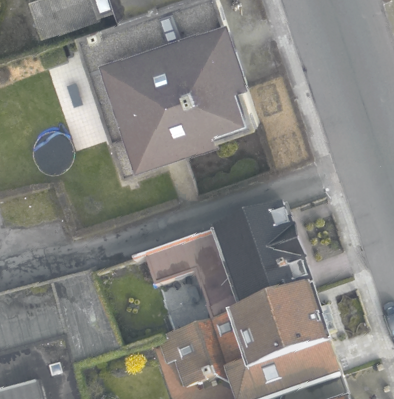
\includegraphics[width=\textwidth]{./Images/DFC2015/optical.png}
      \caption{RGB Modality}
    \end{minipage}
    \begin{minipage}[b]{0.45\linewidth}
      \centering
      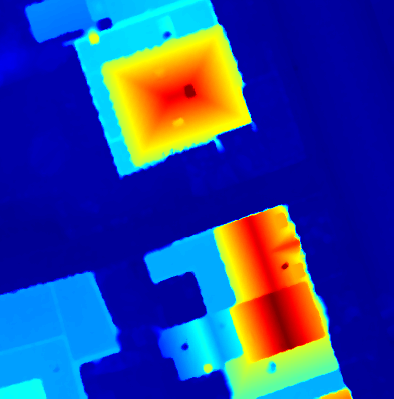
\includegraphics[width=\textwidth]{./Images/DFC2015/lidarColor.png}
      \caption{Lidar Modality}
    \end{minipage}
  \end{figure}
\end{frame}

% ------------------------------------------------

\begin{frame}
  \frametitle{Results}
  \begin{figure}[ht]
    \begin{minipage}[b]{0.3\linewidth}
      \centering
      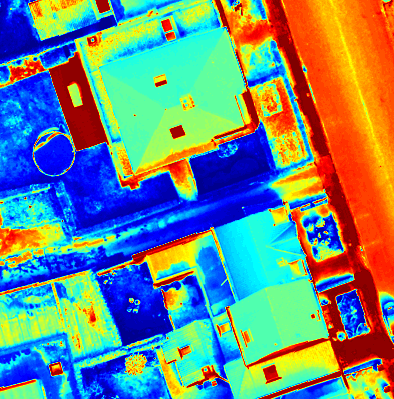
\includegraphics[width=\textwidth]{./Images/DFC2015/evec1.png}
    \end{minipage}
    \begin{minipage}[b]{0.3\linewidth}
      \centering
      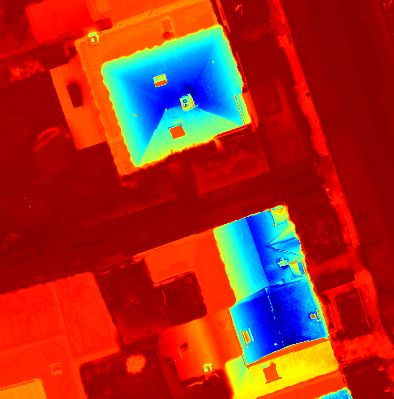
\includegraphics[width=\textwidth]{./Images/DFC2015/evec2.png}
    \end{minipage}
    \begin{minipage}[b]{0.3\linewidth}
      \centering
      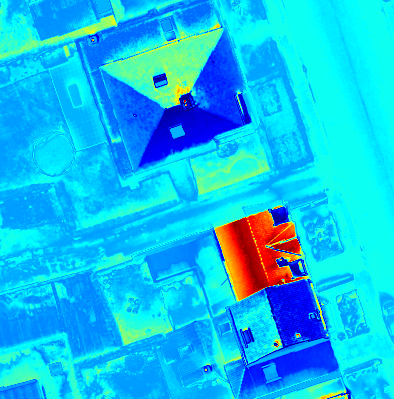
\includegraphics[width=\textwidth]{./Images/DFC2015/evec4.png}
    \end{minipage}
    \caption{Example eigenvectors of graph Laplacian}
  \end{figure}
\end{frame}

% ------------------------------------------------

\begin{frame}
  \frametitle{Results}
  Spectral clustering result (unsupervised). $m = 6$ classes.
  \begin{figure}[ht]
    \begin{minipage}[b]{0.45\linewidth}
      \centering
      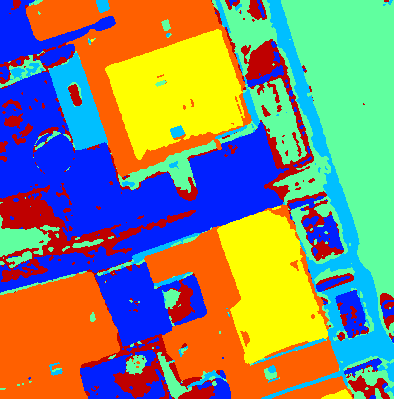
\includegraphics[width=\textwidth]{./Images/DFC2015/K.png}
      \caption{Classes}
    \end{minipage}
    \begin{minipage}[b]{0.45\linewidth}
      \centering
      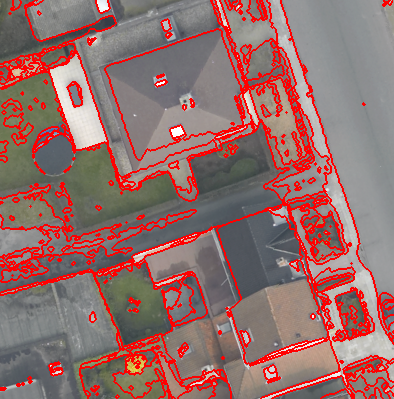
\includegraphics[width=\textwidth]{./Images/DFC2015/segmentation.png}
      \caption{Regions on original image}
    \end{minipage}
  \end{figure}
\end{frame}

% ------------------------------------------------

\begin{frame}
  \frametitle{Results}
  Graph MBO (7\% supervised). $m = 6$ classes.
  \begin{figure}[ht]
    \begin{minipage}[b]{0.45\linewidth}
      \centering
      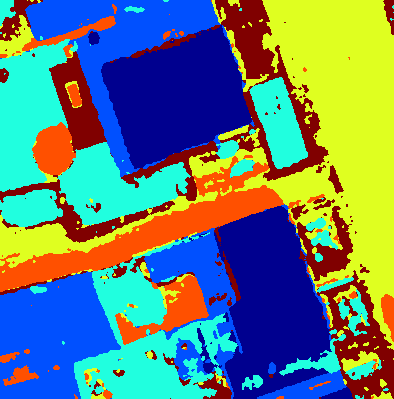
\includegraphics[width=\textwidth]{./Images/DFC2015/MBO/classification.png}
      \caption{Classes}
    \end{minipage}
    \begin{minipage}[b]{0.45\linewidth}
      \centering
      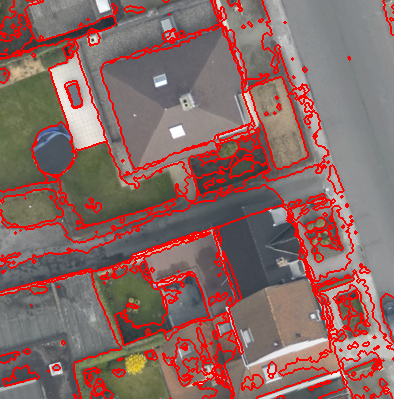
\includegraphics[width=\textwidth]{./Images/DFC2015/MBO/imWithBorders.png}
      \caption{Regions on original image}
    \end{minipage}
  \end{figure}
\end{frame}

% ------------------------------------------------

\begin{frame}
  \frametitle{Umbrella Data}
  Our algorithm applied to \cite{Scharstein2014} dataset.
  \begin{figure}[ht]
    \begin{minipage}[b]{0.45\linewidth}
      \centering
      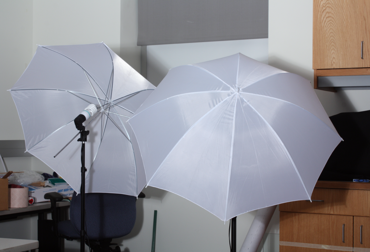
\includegraphics[width=\textwidth]{./Images/Umbrella/optical.png}
      \caption{RGB Modality}
    \end{minipage}
    \begin{minipage}[b]{0.45\linewidth}
      \centering
      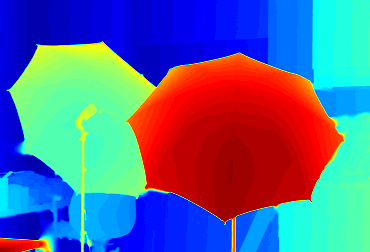
\includegraphics[width=\textwidth]{./Images/Umbrella/lidarColor.png}
      \caption{Lidar Modality}
    \end{minipage}
  \end{figure}
\end{frame}

% ------------------------------------------------

\begin{frame}
  \frametitle{Results}
  \begin{figure}[ht]
    \begin{minipage}[b]{0.40\linewidth}
      \centering
      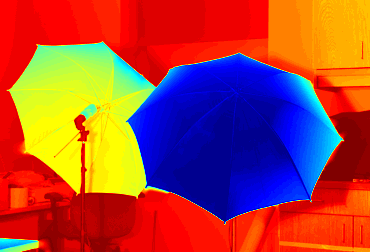
\includegraphics[width=\textwidth]{./Images/Umbrella/evecColor.png}
    \end{minipage}
    \begin{minipage}[b]{0.40\linewidth}
      \centering
      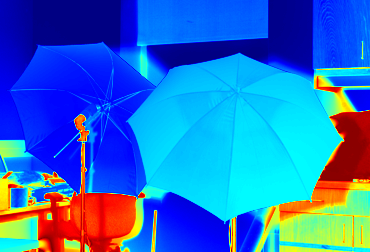
\includegraphics[width=\textwidth]{./Images/Umbrella/evec2.png}
    \end{minipage}
    \vfill
    \begin{minipage}[b]{0.40\linewidth}
      \centering
      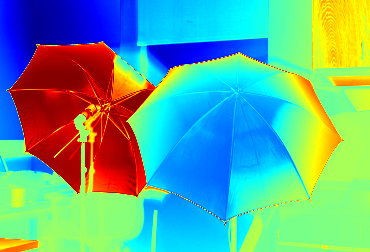
\includegraphics[width=\textwidth]{./Images/Umbrella/evec3.png}
    \end{minipage}
    \caption{Example eigenvectors of graph Laplacian}
  \end{figure}
\end{frame}

% ------------------------------------------------

\begin{frame}
  \frametitle{Results}
  Spectral Clustering result (unsupervised). $m = 6$ classes.
  \begin{figure}[ht]
    \begin{minipage}[b]{0.45\linewidth}
      \centering
      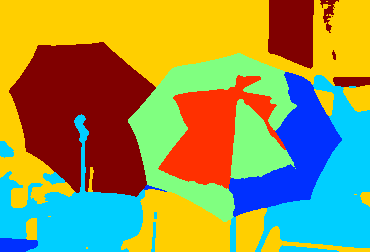
\includegraphics[width=\textwidth]{./Images/Umbrella/classification.png}
      \caption{Classes}
    \end{minipage}
    \begin{minipage}[b]{0.45\linewidth}
      \centering
      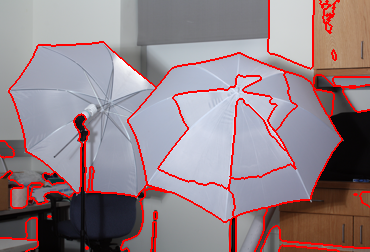
\includegraphics[width=\textwidth]{./Images/Umbrella/imWithBorders.png}
      \caption{Regions on original image}
    \end{minipage}
  \end{figure}
\end{frame}
% ------------------------------------------------

\begin{frame}
  \frametitle{Results}
  Graph MBO result (5\% supervised). $m = 6$ classes.
  \begin{figure}[ht]
    \begin{minipage}[b]{0.45\linewidth}
      \centering
      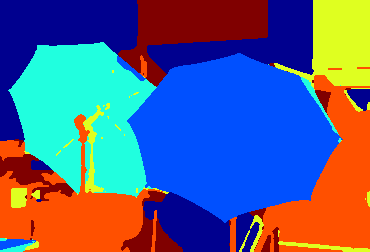
\includegraphics[width=\textwidth]{./Images/Umbrella/MBO/classification.png}
      \caption{Classes}
    \end{minipage}
    \begin{minipage}[b]{0.45\linewidth}
      \centering
      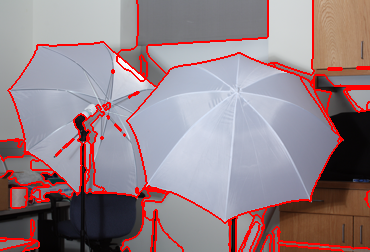
\includegraphics[width=\textwidth]{./Images/Umbrella/MBO/imWithBorders.png}
      \caption{Regions on original image}
    \end{minipage}
  \end{figure}
\end{frame}

% ------------------------------------------------
\section{Graph Matching}
\subsection{Problem Setup}
\begin{frame}
  \frametitle{Graph Matching}
  Goal: Remove or weaken the coregistration assumption.\\
  Create our own registration using topological qualities of data.\\~\\
  %
  View each dataset as a (weighted) graph.\\
  Try to match nodes with similar structure.
  \begin{figure}[ht]
    \centering
    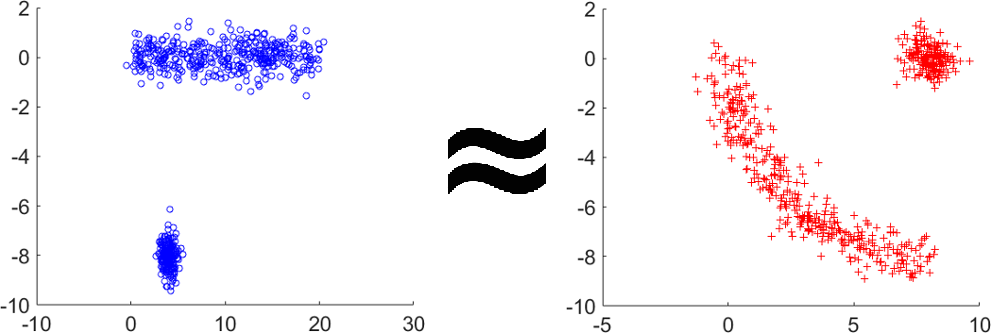
\includegraphics[width=\textwidth]{./Images/GraphMatch/CombinePic/ApproxEq.png}
  \end{figure}  
\end{frame}
% ------------------------------------------------

\begin{frame}
  \frametitle{Problem Setup}
  Two weighted graphs, $G_1,G_2$, with weight matrices $W_1,W_2$.\\~\\
  %
  For convenience of notation, assume $\abs{G_1} = \abs{G_2} = N$.\\~\\
  %
  Search for a graph isomorphism $G_1\to G_2$ preserving edge weights.
  \begin{figure}[ht]
    \centering
    \begin{minipage}[b]{0.40\linewidth}
      \centering
      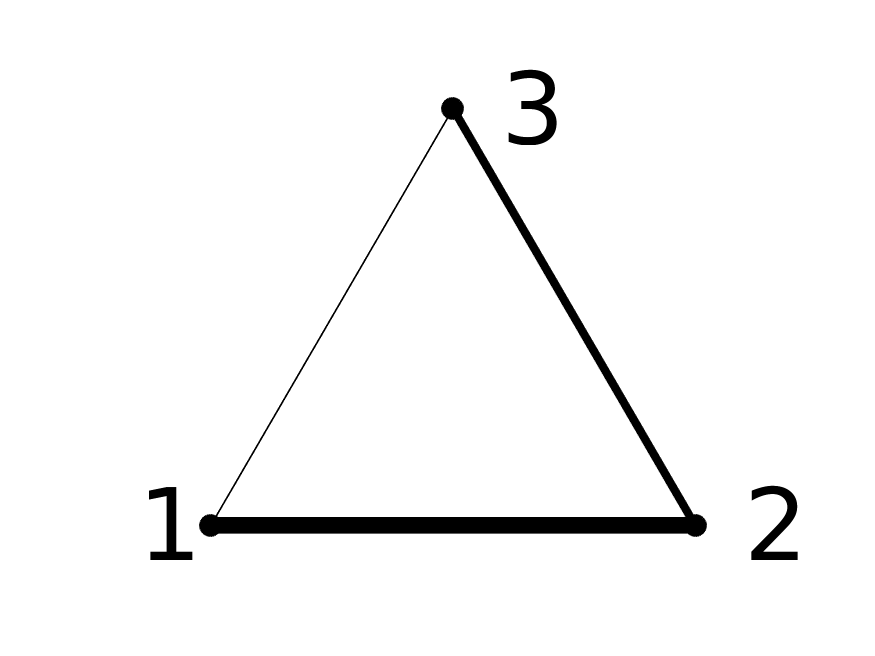
\includegraphics[width=\textwidth]{./Images/GraphMatch/isom1.png}
    \end{minipage}
    \begin{minipage}[b]{0.40\linewidth}
      \centering
      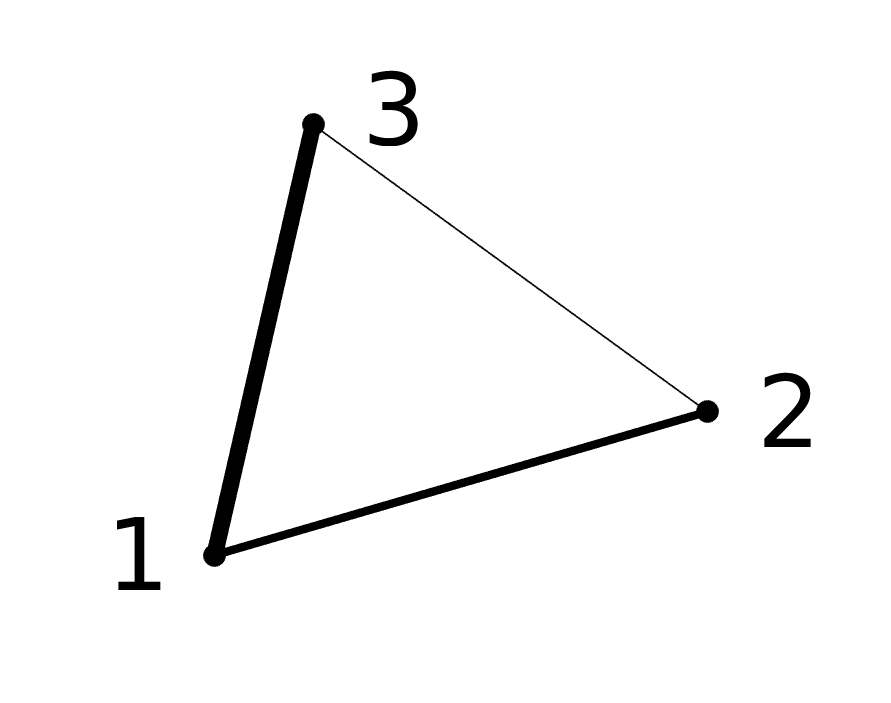
\includegraphics[width=\textwidth]{./Images/GraphMatch/isom2.png}
    \end{minipage}
  \end{figure}
  Best isomorphism is $1 \to 3$, $2 \to 1$, $3 \to 2$.
\end{frame}

% ------------------------------------------------

\begin{frame}
  \frametitle{Problem Setup}
  Isomorphism $G_1\to G_2$ corresponds to a permutation on nodes. Have $P$ the corresponding permutation matrix. Want to find
  \[\text{argmin}_{P\text{ a Permutation matrix}}\norm{W_1 - PW_2P^T}^2_F.\]
  Exact solution is too expensive. Approximate via Graph Laplacian.\\ \cite{Umeyama1988,Knossow2009}.\\~\\
\end{frame}

% ------------------------------------------------

\begin{frame}
  \frametitle{Relaxation}
  Relax problem to
  \[Q^* = \text{argmin}_{QQ^T=I}\norm{W_1 - QW_2Q^T}^2_F.\]
  Let $L_1,L_2$ the graph Laplacians corresponding to $W_1,W_2$ \\~\\
  $U_1,U_2$ the corresponding matrices of eigenvectors. \\~\\
  Then $Q^* = U_1SU_2^T$.\\~\\
  $S$ is diagonal matrix with entries $\pm 1$ to handle sign ambiguity.
\end{frame}

% ------------------------------------------------

\begin{frame}
  \frametitle{Heuristics}
  Recall from Laplacian Theory
  \begin{align*}
    \text{column of }U_i &\iff \text{ feature extracted from data} \\
    \text{row of }U_i &\iff \text{ image of data point in new feature space}.
  \end{align*}
  Match rows of $U_1$ to rows of $U_2$ by considering $U_1U_2^T$. \\~\\
  Currently, $S$ is determined in a semisupervised manner,\\
  align eigenvectors using a few $(< 1\%)$ known matches.
\end{frame}

% ------------------------------------------------

\begin{frame}
  \frametitle{Matching Algorithm}
  $Q^*_{ij}$ gives the similarity between node $i$ of $G_1$ and node $j$ of $G_2$. \\~\\
  %
  Many choices for how to complete the matching:
  \begin{itemize}
  \item Match 1-to-many via maximum similarity.
  \item Match 1-to-1 via \emph{Hungarian Algorithm}.
  \item Match many-to-many via a threshold on $Q^*$.
  \item \textbf{Hierarchical Matching:}\\
    Match some landmark nodes, extend to a full match.\\
    Similar to Nystr\"{o}m, avoid creating the full $N\times N$ graph.
  \end{itemize}
  % Choose a permutation $p: \{1,2,\ldots,N\} \to \{1,2,\ldots,N\}$ via
  % \[\text{argmax}_{\text{permutations }p}\sum_{i=1}^N Q^*_{i,p(i)}.\]
  % Hungarian algorithm finds this in $O(N^3)$ \cite{Munkres1957}.
\end{frame}

% % ------------------------------------------------

% \begin{frame}
%   \frametitle{Benefits of Graph Matching}
%   Benefits of Graph Matching
%   \begin{enumerate}
%   \item Invariant under conformal maps.
%     \begin{itemize}
%     \item scaling, shifts, rotations, etc.
%     \item robust to continuous deformation.
%     \end{itemize}
%   \item A precise number representing similarity between nodes.
%     \begin{itemize}
%     \end{itemize}
%   \item Easy extension to the case $\abs{G_1}\neq\abs{G_2}$.
%   \end{enumerate}
% \end{frame}

% ------------------------------------------------
\begin{frame}
  \frametitle{Example Matching}
  \begin{figure}
    \centering
    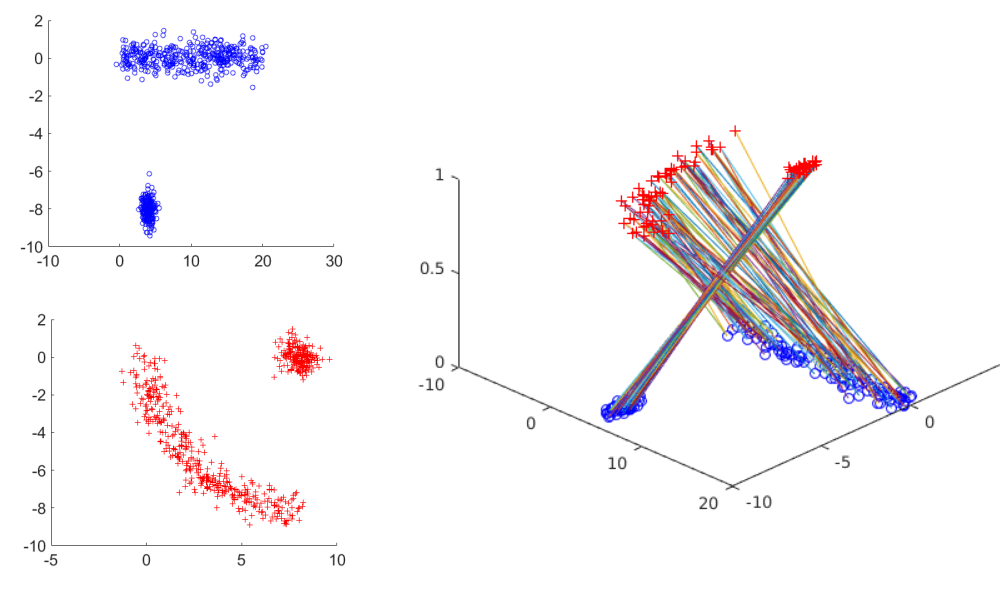
\includegraphics[width = 0.9\textwidth]{./Images/GraphMatch/CombinePic/combinepic.png}
    \caption{Graph Match on Synthetic Data}
  \end{figure}
\end{frame}

% ------------------------------------------------

\subsection{Ideas / Partial Results}
\begin{frame}
  \frametitle{Knowledge Transfer}
  Knowledge transfer via Graph Matching.
  \begin{itemize}
  \item 2 hyperspectral images. 68 bands. (ARTEMISAT-2 Project)
  \item Area 1 is segmented into 6 classes. (Given with data)
  \item Match Area 1 to Area 2. Transfer classification via match.
  \end{itemize}
  \begin{figure}[ht]
    \centering
    \begin{minipage}[b]{0.30\linewidth}
      \centering
      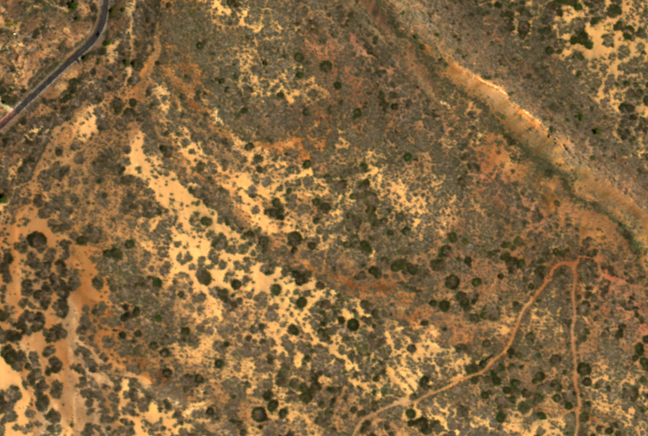
\includegraphics[width=\textwidth]{./Images/EdurneAreas/Area2.png}
      \caption{Area 1 (RGB bands)}
    \end{minipage}
    \hfill
    \begin{minipage}[b]{0.30\linewidth}
      \centering
      \includegraphics[width=\textwidth]{./Images/EdurneAreas/Area2OriginalClassification.png}
      \caption{Area 1 Classification}
    \end{minipage}
    \hfill
    \begin{minipage}[b]{0.30\linewidth}
      \centering
      \includegraphics[width=\textwidth]{./Images/EdurneAreas/Area1.png}
      \caption{Area 2 (RGB bands)}
    \end{minipage}
  \end{figure}      
\end{frame}

% ------------------------------------------------

\begin{frame}
  \frametitle{Knowledge Transfer}
  Correctly classify 72\% of pixels.
  \begin{figure}[ht]
    \centering
    \begin{minipage}[b]{0.48\linewidth}
      \centering
      \includegraphics[width=\textwidth]{./Images/EdurneAreas/Area1GraphTransferClassification.png}
      \caption{Transfer to Area 2}
    \end{minipage}
    \hfill
    \begin{minipage}[b]{0.48\linewidth}
      \centering
      \includegraphics[width=\textwidth]{./Images/EdurneAreas/Area1OriginalClassification.png}
      \caption{Area 2 Ground Truth}
    \end{minipage}
  \end{figure}
\end{frame}

% ------------------------------------------------

\begin{frame}
  \frametitle{Change Detection}
  Change detection via Graph Matching:\\~\\
  %
  Given \emph{coregistered} data $X$ and $Y$, compare the match via registration against the match via graphs.\\~\\
  % 
  From graph matching, get a permutation
  \[\rho: \{1,\ldots,n\} \to \{1,\ldots,n\}.\]
  % 
  Look at $\norm{x_i-x_{\rho^{-1}(i)}}$ and $\norm{y_i - y_{\rho(i)}}$. \\~\\
\end{frame}

% ------------------------------------------------

\begin{frame}
  \frametitle{Change Detection Example}
  Flood data: Data Fusion Contest 2010 \cite{Longbotham2012}.\\~\\
  SPOT Satellite images before and after flood.\\
  3 bands, near-infrared (displayed in false color).
  \begin{figure}[ht]
    \centering
    \hfill
    \begin{minipage}[b]{0.40\linewidth}
      \centering
      \includegraphics[width=\textwidth]{./Images/ChangeDetect/Flood/pictureX.png}
      \caption{Before Flood}
    \end{minipage}
    \hfill
    \begin{minipage}[b]{0.40\linewidth}
      \centering
      \includegraphics[width=\textwidth]{./Images/ChangeDetect/Flood/pictureY.png}
      \caption{After Flood}
    \end{minipage}
    \hfill
  \end{figure}
\end{frame}

% ------------------------------------------------

\begin{frame}
  \frametitle{Change Detection Example}
  \setlength{\abovecaptionskip}{0pt plus 0pt minus 2pt} % Chosen fairly arbitrarily
  \begin{figure}[ht]
    \centering
    \begin{minipage}[b]{0.28\linewidth}
      \centering
      \includegraphics[width=\textwidth]{./Images/ChangeDetect/Flood/pictureX.png}
      \caption{Data $X$}
    \end{minipage}
    \hfill
    \begin{minipage}[b]{0.28\linewidth}
      \centering
      \includegraphics[width=\textwidth]{./Images/ChangeDetect/Flood/permX.png}
      \caption{Approx $Y$ by $X$}
    \end{minipage}
    \hfill
    \begin{minipage}[b]{0.28\linewidth}
      \centering
      \includegraphics[width=\textwidth]{./Images/ChangeDetect/Flood/ChangesXtoY.png}
      \caption{$\norm{X - \text{perm}(X)}$}
    \end{minipage}
    \begin{minipage}[b]{0.28\linewidth}
      \centering
      \includegraphics[width=\textwidth]{./Images/ChangeDetect/Flood/pictureY.png}
      \caption{Data $Y$}
    \end{minipage}
    \hfill
    \begin{minipage}[b]{0.28\linewidth}
      \centering
      \includegraphics[width=\textwidth]{./Images/ChangeDetect/Flood/permY.png}
      \caption{Approx $X$ by $Y$}
    \end{minipage}
    \hfill
    \begin{minipage}[b]{0.28\linewidth}
      \centering
      \includegraphics[width=\textwidth]{./Images/ChangeDetect/Flood/ChangesYtoX.png}
      \caption{$\norm{Y-\text{perm}(Y)}$}
    \end{minipage}
  \end{figure}  
\end{frame}

% ------------------------------------------------

\begin{frame}
  \frametitle{Change Detection}
  Change detection to find unique information in different modalities.\\~\\
  Synthetic Example: 1-D observations over time.
  \begin{figure}[ht]
    \centering
    \begin{minipage}[b]{0.45\linewidth}
      \centering
      \includegraphics[width=\textwidth]{./Images/ChangeDetect/Synthetic/data.png}
      \caption{Input Data}
    \end{minipage}
    \hfill
      \begin{minipage}[b]{0.45\linewidth}
      \centering
      \includegraphics[width=\textwidth]{./Images/ChangeDetect/Synthetic/norms.png}
      \caption{Norm Comparison (scaled)}
    \end{minipage}
  \end{figure}
\end{frame}

% ------------------------------------------------

\begin{frame}
  Change detection to find unique information in different modalities.
  \begin{figure}[ht]
    \centering
    \begin{minipage}[b]{0.32\linewidth}
      \centering
      \includegraphics[width=\textwidth]{./Images/ChangeDetect/JadePlant/pictureX.png}
      \caption{Data $X$}
    \end{minipage}
    \hfill
    \begin{minipage}[b]{0.32\linewidth}
      \centering
      \includegraphics[width=\textwidth]{./Images/ChangeDetect/JadePlant/permX.png}
      \caption{Approx $Y$ by $X$}
    \end{minipage}
    \hfill
    \begin{minipage}[b]{0.32\linewidth}
      \centering
      \includegraphics[width=\textwidth]{./Images/ChangeDetect/JadePlant/ChangesXtoY.png}
      \caption{$\norm{X - \text{perm}(X)}$}
    \end{minipage}
    \begin{minipage}[b]{0.32\linewidth}
      \centering
      \includegraphics[width=\textwidth]{./Images/ChangeDetect/JadePlant/pictureY.png}
      \caption{Data $Y$}
    \end{minipage}
    \hfill
    \begin{minipage}[b]{0.32\linewidth}
      \centering
      \includegraphics[width=\textwidth]{./Images/ChangeDetect/JadePlant/permY.png}
      \caption{Approx $X$ by $Y$}
    \end{minipage}
    \hfill
    \begin{minipage}[b]{0.32\linewidth}
      \centering
      \includegraphics[width=\textwidth]{./Images/ChangeDetect/JadePlant/ChangesYtoX.png}
      \caption{$\norm{Y-\text{perm}(Y)}$}
    \end{minipage}
  \end{figure}  
\end{frame}
% ------------------------------------------------

\section{References}
\begin{frame}[allowframebreaks]
  \frametitle{References}
  \footnotesize{
    \begin{thebibliography}{99} % Beamer does not support BibTeX so references must be inserted manually as below
    \bibitem[Longbotham et al, IEEE,2012]{Longbotham2012} Longbotham, Nathan and Pacifici, Fabio and Glenn, Taylor and Zare, Alina and Volpi, Michele and Tuia, Devis and Christophe, Emmanuel and Michel, Julien and Inglada, Jordi and Chanussot, Jocelyn and Du, Qian
      \newblock Multi-modal change detection, application to the detection of flooded areas: outcome of the 2009-2010 data fusion contest
      \newblock \emph{IEEE J. Sel. Topics Appl. Earth Observ.} 5(1):331-342
    \bibitem[Chung, AMS, 1997]{Chung1997} Fan R. K. Chung
      \newblock Spectral Graph Theory
      \newblock CBMS Reg. Conf. Ser. Math. 92, Providence, RI, 1997
      % 
      % 
    \bibitem[Mertens et al, CGF, 2008]{Mertens2008} Tom Mertens and J. Kautz and Frank Van Reeth
      \newblock Exposure Fusion: A Simple and Practical Alternative to High Dynamic Range Photography
      \newblock \emph{Computer Graphics Forum} 28(1):161 - 171
      % 
      % 
    \bibitem[Datcu et al, IEEE CVPR 2007]{Dactu2007} D. Datcu and Z. Yang and L. Rothkrantz (2007)
      \newblock Multimodal workbench for automatic surveillance applications
      \newblock \emph{2007 IEEE Conference on Computer Vision and Pattern Recognition} 1-2
      % 
      % 
    \bibitem[Lahat et al, IEEE 2015]{Lahat2015} Lahat, Dana and Adal{\i}, T{\"u}lay and Jutten, Christian (2015)
      \newblock Multimodal Data Fusion: An Overview of Methods, Challenges and Prospects
      \newblock \emph{Proceedings of the IEEE } 103(9), 1449-1477
      % 
      % 
    \bibitem[Yeh et al, IEEE TIP 2014]{Yeh2014} Yi-Ren Yes and Chun-Hao Huang and Yu-Chiang Frank Wang
      \newblock Heterogeneous Domain Adaptation and Classification by Exploiting the Correlation Subspace
      \newblock \emph{IEEE Transactions on Image Processing} 23(5), 2009-2018
      % 
      % 
    \bibitem[Wang et al, IJCAI 2013]{Wang2013} Wang, Chang and Mahadevan, Sridhar (2013)
      \newblock Manifold Alignment Preserving Global Geometry
      \newblock \emph{Proceedings of the Twenty-Third International Joint Conference on Artificial Intelligence} IJCAI '13, 1743-1749
      % 
      % 
    \bibitem[Tuia et al, PLOS ONE 2016]{Tuia2016} Tuia, Devis AND Camps-Valls, Gustau (2016)
      \newblock Kernal Manifold Alignment for Domain Adaptation
      \newblock \emph{PLOS ONE} 11, 1-25
      %
      %
    \bibitem[Bampos-Taberner et al, IEEE J-STARS 2016]{DFC2015} M. Campos-Taberner and A. Romero-Soriano and C. Gatta and G. Camps-Valls and A. Lagrange and B. Le Saux and A. Beaupère and A. Boulch and A. Chan-Hon-Tong and S. Herbin and H. Randrianarivo and M. Ferecatu and M. Shimoni and G. Moser and D. Tuia (2015)
      \newblock Processing of Extremely High-Resolution LiDAR and RGB Data: Outcome of the 2015 IEEE GRSS Data Fusion Contest \#8211;Part A: 2-D Contest
      \newblock \emph{IEEE Journal of Selected Topics in Applied Earth Observations and Remote Sensing} 9(12), 5547-5559
      %
      %
    \bibitem[Iyer et al., ICIP 2017]{Iyer2017} Iyer, Geoffrey and Chanussot, Jocelyn and Bertozzi, Andrea (2017).
      \newblock A Graph-Based Approach for Feature Extraction and Segmentation of Multimodal Images
      \newblock Preprint
      %
      %
    \bibitem[Scharstein et al., GCPR 2014]{Scharstein2014} Daniel Scharstein and Heiko Hirschm\"{u}ller and York Kitajima and Greg Krathwohl and Nera Ne\v{s}i\'{c} and Xi Wang and Porter Westling (2014)
      \newblock High-resolution stereo datasets with subpixel-accurate ground truth
      \newblock \emph{Proceedings of the 36th German Conference on Pattern Recognition} 31-42
      %
      %
    \bibitem[Umeyama, IEEE TPAMI 1988]{Umeyama1988} Umeyama, S. (1988)
      \newblock An Eigendecomposition Approach to Weighted Graph Matching Problems
      \newblock \emph{IEEE Trans. Pattern Anal. Mach. Intell.}, 10(5), 695-703
      %
      %
    \bibitem[Knossow et al., GbRPR 2009]{Knossow2009} Knossow, David and Sharma, Avinash and Mateus, Diana and Horaud, Radu (2009)
      \newblock Inexact Matching of Large and Sparse Graphs Using Laplacian Eigenvectors
      \newblock Graph-Based Representations in Pattern Recognition: 7th IAPR-TC-15 International Workshop, 2009. Proceedings
      %
      %
    \bibitem[vonLuxburg, Stat Comput 2007]{vonLuxburg07} vonLuxburg, Ulrike (2007)
      \newblock A tutorial on spectral clustering
      \newblock Statistics and Computing, 17(4), 395-416
      %
      %
    \bibitem[Merkurjev, SIIMS 2013]{Merkurjev13} Ekaterina Merkurjev and Tijana Kostic and Andrea L Bertozzi (2013)
      \newblock An MBO scheme on graphs for classification and image processing
      \newblock SIAM Journal on Imaging Sciences, 6(4), 1903-1930
      %
      %
    \bibitem[Fowlkes et al., IEEE TPAMI 2004]{Fowlkes04} Charless Fowlkes and Serge Belongie and Fan Chung and Jitendra Malik (2004)
      \newblock Spectral Grouping Using the Nystrom Method
      \newblock IEEE Transactions on Pattern Analysis and Machine Intelligence, 26(2)
      %
      %
    \bibitem[Munkres, SIAM 1957]{Munkres1957} J. Munkres (1957)
      \newblock Algorithms for the Assignment and Transportation Problems
      \newblock Journal of the Society for Industrial and Applied Mathematics, 5(1):32–38
    \end{thebibliography}
  }
\end{frame}

% ------------------------------------------------

\begin{frame}
\frametitle{Hungarian Algorithm}
  Say we have $N=6$ and calculated:
  \[Q^* = \begin{pmatrix}
   -0.1629 &  -0.1711 &  -0.1703 &   0.3426 &   0.3717 &  -0.2100\\
   -0.1647 &  -0.1662 &  -0.1677 &   0.2966 &   0.3192 &  -0.1172\\
   -0.1660 &  -0.1653 &  -0.1657 &  -0.1477 &  -0.1861 &   0.8308\\
   -0.4579 &   0.6860 &   0.2665 &  -0.1787 &  -0.1480 &  -0.1678\\
    0.4939 &  -0.1039 &   0.1196 &  -0.6689 &   0.3080 &  -0.1486\\
    0.4577 &  -0.0795 &   0.1176 &   0.3561 &  -0.6647 &  -0.1872\\
  \end{pmatrix}\]
  Then \[P^* = \begin{pmatrix}
      0&0&0&1&0&0\\
      0&0&0&0&1&0\\
      0&0&0&0&0&1\\
      0&1&0&0&0&0\\
      1&0&0&0&0&0\\
      0&0&1&0&0&0\\
    \end{pmatrix}
  \]
\end{frame}

% ------------------------------------------------

\begin{frame}
  \frametitle{Graph Matching Example}
  \begin{figure}[ht]
    \centering
    \begin{minipage}[b]{0.40\linewidth}
      \centering
      \includegraphics[width=\textwidth]{./Images/GraphMatch/structureEx1.png}
      \caption{Graph 1}
    \end{minipage}
    \begin{minipage}[b]{0.40\linewidth}
      \centering
      \includegraphics[width=\textwidth]{./Images/GraphMatch/structureEx2.png}
      \caption{Graph 2}
    \end{minipage}
  \end{figure}
  Any reasonable matching sends $1 \to 2$. \\~\\
  %
  Other nodes can be matched in many ways (symmetry).
\end{frame}

% ------------------------------------------------

\begin{frame}
  \frametitle{Change Detection Example 2}
  Synthetic Example: Graph representation is useful!\\~\\
  Continuous transform ($\mathbb{R}^3 \to \mathbb{R}^3$) applied to most pixels,\\
  One extra artifact added.\\
  Simulate data captured from different sources.
  \begin{figure}[ht]
    \centering
    \begin{minipage}[b]{0.32\linewidth}
      \centering
      \includegraphics[width=\textwidth]{./Images/ChangeDetect/ChairArtifact/pictureX.png}
      \caption{Original Picture}
    \end{minipage}
    \hfill
    \begin{minipage}[b]{0.32\linewidth}
      \centering
      \includegraphics[width=\textwidth]{./Images/ChangeDetect/ChairArtifact/pictureY.png}
      \caption{Altered Picture}
    \end{minipage}
    \hfill
    \begin{minipage}[b]{0.32\linewidth}
      \centering
      \includegraphics[width=\textwidth]{./Images/ChangeDetect/ChairArtifact/ChangesXtoY.png}
      \caption{Norm Comparison}
    \end{minipage}
  \end{figure}
\end{frame}

% ------------------------------------------------

\begin{frame}
  \frametitle{Change Detection Example}
  \begin{figure}
    \begin{minipage}[b]{0.40\linewidth}
      \centering
      \includegraphics[width=\textwidth]{./Images/GraphMatch/dataAfter.png}
      \caption{Image $X$}
    \end{minipage}
    \hfill
    \begin{minipage}[b]{0.40\linewidth}
      \centering
      \includegraphics[width=\textwidth]{./Images/GraphMatch/dataBefore.png}
      \caption{Image $Y$}
    \end{minipage}
    \vfill
    \begin{minipage}[b]{0.40\linewidth}
      \centering
      \includegraphics[width=\textwidth]{./Images/GraphMatch/naivediff.png}
      \caption{Naive difference $\norm{X-Y}$}
    \end{minipage}
    \hfill
    \begin{minipage}[b]{0.40\linewidth}
      \centering
      \includegraphics[width=\textwidth]{./Images/GraphMatch/normMap.png}
      \caption{$\norm{x_i - x_{\rho(i)}}$}
    \end{minipage}
  \end{figure}
\end{frame}


% % ------------------------------------------------
  
% \begin{frame}
%   \frametitle{Blocks of Highlighted Text}
%   \begin{block}{Block 1}
%     Lorem ipsum dolor sit amet, consectetur adipiscing elit. Integer lectus nisl, ultricies in feugiat rutrum, porttitor sit amet augue. Aliquam ut tortor mauris. Sed volutpat ante purus, quis accumsan dolor.
%   \end{block}

%   \begin{block}{Block 2}
%     Pellentesque sed tellus purus. Class aptent taciti sociosqu ad litora torquent per conubia nostra, per inceptos himenaeos. Vestibulum quis magna at risus dictum tempor eu vitae velit.
%   \end{block}

%   \begin{block}{Block 3}
%     Suspendisse tincidunt sagittis gravida. Curabitur condimentum, enim sed venenatis rutrum, ipsum neque consectetur orci, sed blandit justo nisi ac lacus.
%   \end{block}
% \end{frame}

% % ------------------------------------------------

% \begin{frame}
%   \frametitle{Multiple Columns}
%   \begin{columns}[c] % The "c" option specifies centered vertical alignment while the "t" option is used for top vertical alignment

%     \column{.45\textwidth} % Left column and width
%     \textbf{Heading}
%     \begin{enumerate}
%     \item Statement
%     \item Explanation
%     \item Example
%     \end{enumerate}

%     \column{.5\textwidth} % Right column and width
%     Lorem ipsum dolor sit amet, consectetur adipiscing elit. Integer lectus nisl, ultricies in feugiat rutrum, porttitor sit amet augue. Aliquam ut tortor mauris. Sed volutpat ante purus, quis accumsan dolor.

%   \end{columns}
% \end{frame}

% % ------------------------------------------------

% \begin{frame}
%   \frametitle{Table}
%   \begin{table}
%     \begin{tabular}{l l l}
%       \toprule
%       \textbf{Treatments} & \textbf{Response 1} & \textbf{Response 2}\\
%       \midrule
%       Treatment 1 & 0.0003262 & 0.562 \\
%       Treatment 2 & 0.0015681 & 0.910 \\
%       Treatment 3 & 0.0009271 & 0.296 \\
%       \bottomrule
%     \end{tabular}
%     \caption{Table caption}
%   \end{table}
% \end{frame}

% % ------------------------------------------------

% \begin{frame}
%   \frametitle{Theorem}
%   \begin{theorem}[Mass--energy equivalence]
%     $E = mc^2$
%   \end{theorem}
% \end{frame}

% % ------------------------------------------------

% \begin{frame}[fragile] % Need to use the fragile option when verbatim is used in the slide
%   \frametitle{Verbatim}
%   \begin{example}[Theorem Slide Code]
% \begin{verbatim}
% \begin{frame}
%   \frametitle{Theorem}
%   \begin{theorem}[Mass--energy equivalence]
%     $E = mc^2$
%   \end{theorem}
% \end{verbatim}
% \end{example}
% \end{frame}

% \begin{frame}[fragile] % Need to use the fragile option when verbatim is used in the slide
%   \frametitle{Citation}
%   An example of the \verb|\cite| command to cite within the presentation:\\~

%   This statement requires citation NOT ANYMORE I COMMENTED IT OUT HAHAHA%\cite{p1}.
% \end{frame}

% ------------------------------------------------

\end{document}